\documentclass[12pt]{article}
\usepackage{amsmath,amssymb}
\usepackage{geometry}
\geometry{margin=1in}
\usepackage[hidelinks]{hyperref}
\setlength{\parindent}{0pt}
\usepackage{xcolor}
\usepackage{etoolbox}  %Supports toggle commands
\definecolor{darkblue}{RGB}{0,0,139}
\usepackage{graphicx}

%SETTINGS
\newtoggle{solutions} \togglefalse{solutions}

\begin{document}

\begin{center}
\textbf{Week 10 - Review Session} \\
Introduction to Health Economics: EC 387 \\
Boston University \\
Spring 2026 \\
Professor Pauline Mourot
\end{center}

\vspace{1em}

\noindent \textbf{Exercise 1: TRUE/FALSE/UNCERTAIN}\\

For each of the questions below, please explain your answer.
The quality of the explanation is an important part of the grade for these problems and
can also help you earn substantial partial credit.
In answering each question, 1-3 sentences of explanation should be sufficient.

\vspace{7mm}

\begin{enumerate}
    %\item In spite of the theory, there is limited evidence that adverse selection exists in health insurance markets.

    \item Though health insurers could use contract features to attract or ``screen'' which consumers purchase their plans,
    this is likely very hard to do and there is very limited evidence for this in practice.

    \vspace{3mm}
    \iftoggle{solutions}{
        { \color{darkblue}

        FALSE. We have seen in class a research paper showing that health insurers manipulate their drug formularies to attract more profitable patients.
        
    }}{}

    \item The individual mandate was successfully implemented in the Affordable Care Act (ACA).

    \vspace{3mm}
    \iftoggle{solutions}{
        { \color{darkblue}

        FALSE. The individual mandate was implemented but the tax penalty was probably too low to be effective, and it was repealed in 2017.
        
    }}{}

    \item The regulation on health insurance market exchanges exacerbated the issue of adverse selection for health insurers in the ACA,
    and this led to the collapse of the health insurance market exchanges in the ACA.

    \vspace{3mm}
    \iftoggle{solutions}{
        { \color{darkblue}

        FALSE. It is true that the regulation on health insurance market exchanges exacerbated the issue of adverse selection for health insurers in the ACA,
        because it prevented health insurers to give different prices to different consumers based on their health status notably,
        so asymmetry of information was more severe.
        However, the ACA also implemented the individual mandate, which was designed to mitigate the issue of adverse selection by encouraging healthy people to purchase insurance.
        It also implemented several payments to health insurers to compensate them for enrolling sicker people, such as risk adjustment payments, reinsurance payments, and risk corridor payments.
        
    }}{}

    \item Health insurance has no impact on people beyond just their health care utilization.

    \vspace{3mm}
    \iftoggle{solutions}{
        { \color{darkblue}

        FALSE. It has an impact on financial health and on mortality.
        
    }}{}

    \item You can estimate the impact of health insurance on mortality by comparing the mortality rates of people with and without health insurance.

    \vspace{3mm}
    \iftoggle{solutions}{
        { \color{darkblue}

        FALSE. There is an issue of selection into health insurance, so people with and without health insurance are not comparable.
        In particular, we expect people with health insurance to be sicker on average than people without health insurance,
        which could lead to find a higher mortality rate among people with health insurance than among people without health insurance.
        This would not be because health insurance increases mortality, but because people with health insurance are sicker on average than people without health insurance.
        To address this issue, we need to use a research design that allows us to compare people with and without health insurance who are similar in terms of their health status.
        We have seen in class that RCTs, difference-in-difference approaches, regression discontinutity designs, or instrumental variable approaches can be used to address this issue of selection into health insurance
        and to estimate the causal impact of health insurance on mortality.
        
    }}{}


    \item There is evidence that health insurers shift the cost of having to care for uninsured patients to insured patients by charging higher prices to insured patients.

    \vspace{3mm}
    \iftoggle{solutions}{
        { \color{darkblue}

        FALSE. We have seen a research paper in class that estimated the impact of higher uninsured rates on hospitals costs and profit margins.
        This study found that higher uninsured rates lead to higher costs and lower profit margins for hospitals,
        which is inconsistent with cost-shifting.
        
    }}{}

    \item Uninsurance leads to many patients being denied care in hospitals.

    \vspace{3mm}
    \iftoggle{solutions}{
        { \color{darkblue}

        FALSE/UNCERTAIN. The Emergency Medical Treatment and Labor Act (EMTALA) requires hospitals to provide emergency care to all patients regardless of their insurance status,\
        so hospitals cannot refuse to treat uninsured patients in emergency situations. However, the care they are required to provide under EMTALA is limited to emergency care,
        so they can refuse to treat uninsured patients in non-emergency situations.
        Also, the status of hospitals as non-profits and medical ethics tends to limit such practices, to some extent.
        
    }}{}

\end{enumerate}

\clearpage

\noindent \textbf{Exercise 2:}\\
Consider the market for a given health insurance product, as depicted below.
If consumers do not purchase this health insurance product, they remain uninsured.

\begin{center}
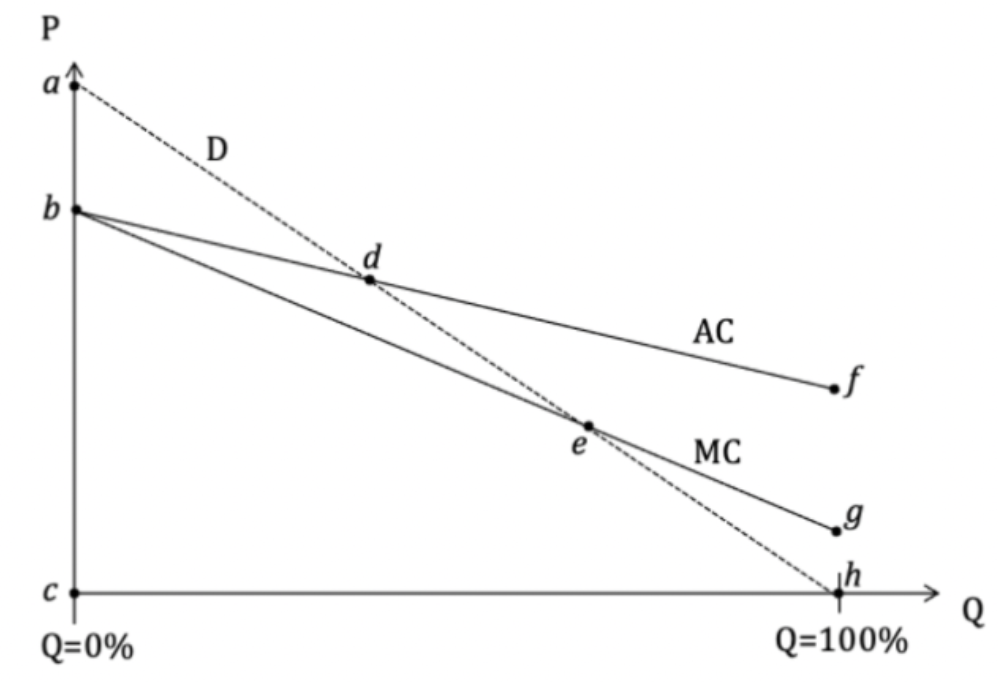
\includegraphics[width=0.6\textwidth]{input/graphex2.png}
\end{center}
 
\begin{enumerate}
    \item[(a)] Which point represents the competitive equilibrium allocation? 

    \vspace{3mm}
    \iftoggle{solutions}{
        { \color{darkblue}

    Point d, the competitive equilibrium is where price = average cost.
    You can obtain this by setting profits to zero: P*Q - AC*Q = 0, which implies P = AC.

    }}{}

    \item[(b)] At the competitive equilibrium allocation, do insurers make positive, negative, or zero profits on the last (i.e. the marginal) consumer that purchases insurance?

        \vspace{3mm}
    \iftoggle{solutions}{
        { \color{darkblue}

    Positive profits, the competitive equilibrium price is higher than the marginal cost.

    }}{}

    \item[(c)] At the competitive equilibrium allocation, do insurers make positive, negative, or zero profits on the consumers with the highest willingness-to-pay in the market?
    What vertical distance represents the profits insurers make on these highest-WTP consumers? 

    \vspace{3mm}
    \iftoggle{solutions}{
        { \color{darkblue}

    They make negative profits on the highest WTP consumer, because the competitive equilibrium price is lower that the WTP for this consumer.
    The vertical distance between the price at point b and the competitive price (price point from point d) indicates this negative profit on this consumer.

    }}{}


    \item[(d)] What are insurers' total profits at the competitive equilibrium? 

        \vspace{3mm}
    \iftoggle{solutions}{
        { \color{darkblue}

    They make zero profit. This is because the competitive equilibrium price is equal to average cost, so profits are zero for all consumers.
    You can see this with using 
    \begin{align*}
    \text{Profits} &= P*Q - AC*Q \\
    &= (P - AC)*Q \\
    &= (AC - AC)*Q \\
    &= 0
    \end{align*}
    }}{}
    \item[(e)] What point represents the socially efficient allocation? 

    \vspace{3mm}
    \iftoggle{solutions}{
        { \color{darkblue}

    Point e indicates the socially efficient allocation where marginal cost = demand (marginal benefit)
    point d) indicates this negative profit on this consumer.

    }}{}

    \item[(f)] What might be a reason that it is not socially efficient for some consumers in the market not to have insurance? 

    \vspace{3mm}
    \iftoggle{solutions}{
        { \color{darkblue}

    This could be due to the existence of moral hazard, or because providing insurance creates administrative costs (loading).

    }}{}


    \item[(g)] What would insurers' total profits be at the socially efficient allocation? 

    \vspace{3mm}
    \iftoggle{solutions}{
        { \color{darkblue}

    Consumers would pay a price equal to the marginal cost at the socially efficient allocation and we would have the quantity of insurance equal to the socially efficient quantity.
    The total revenue would be equal to the rectangle area with height $p^{efficient}$ and width $Q^{efficient}$.
    But what would be the total costs for the insurer at this allocation?
    The average cost at the socially efficient quantity is higher than $p^{efficient}$.
    The total cost would be the average cost at the socially efficient quantity times the quantity of insurance at the socially efficient allocation,
    which is equal to the rectangle area with height AC at $Q^{efficient}$ and width $Q^{efficient}$.
    This means that total costs are larger than total revenue at the socially efficient allocation, so insurers would make negative profits at this allocation.
    This negative profit would be equal to the difference between total revenue and total costs,
    which is equal to the area of the rectangle with width $Q^{efficient}$ and height equal to the vertical distance between AC and MC at $Q^{efficient}$ (red rectangle in the graph).
    }}{}

    \item[(h)] What area represents social surplus at the socially efficient allocation? 

    \vspace{3mm}
    \iftoggle{solutions}{
        { \color{darkblue}
    The triangle abe.
    }}{}

    \item[(i)] Now assume only a single insurer can operate in this market (i.e. the market is a monopoly).
    What would be the new equilibrium price and quantity in this market?
    Describe how you would proceed to find this new equilibrium price and quantity, but you do not need to calculate the exact values.

    \vspace{3mm}
    \iftoggle{solutions}{
        { \color{darkblue}
    
    With a monopolist, we know that the new equilibrium will be where marginal revenue = marginal cost.
    To find the new equilibrium price and quantity, we would first need to derive the marginal revenue curve from the demand curve,
    and then find the point where this marginal revenue curve intersects the marginal cost curve. 

    To obtain the marginal revenue curve, we would compute the total revenue (TR) as a function of quantity (Q) using the demand curve,
    and then take the derivative of total revenue with respect to quantity to get marginal revenue (MR).
    \begin{align*}
    TR(Q) &= P(Q) * Q \\
    MR(Q) &= \frac{\partial TR}{\partial Q}
    \end{align*}

    Then we would solve for $Q^M$ such that $MR(Q^M) = MC(Q^M)$, where $MC(Q)$ is the marginal cost curve.
    To get the monopoly price,
    we would plug this quantity $Q^M$ into the demand curve to find the corresponding price $P^M$.
    }}{}

    \item[(j)] Would the number of consumers purchasing insurance increase, decrease, or stay the same when the market changes from a competitive market to a monopoly in this case?

     \vspace{3mm}
    \iftoggle{solutions}{
        { \color{darkblue}

    The number of consumers purchasing insurance would decrease, because the monopolist will charge a higher price than the competitive equilibrium price, which will lead to a lower quantity demanded.


    \begin{center}
        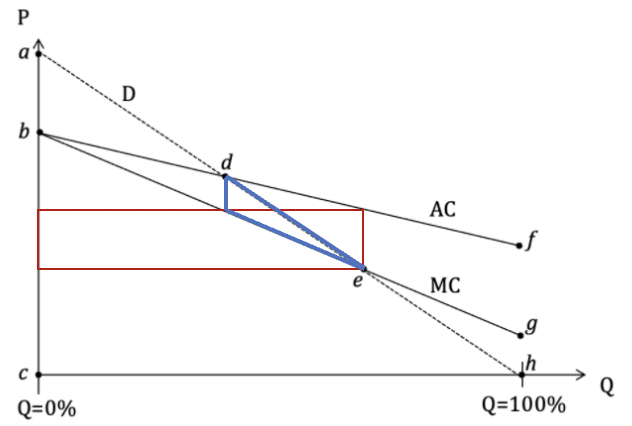
\includegraphics[width=0.6\textwidth]{input/graphex2solution.png}
    \end{center}

    }}{}

    \item[(k)] How would the graph above change if you were told there was advantageous selection in this market? Explain.

     \vspace{3mm}
    \iftoggle{solutions}{
        { \color{darkblue}

    The marginal cost curve would be increasing in quantity, because with advantageous selection,
    the consumers with the highest willingness-to-pay are also those with the lowest costs for the insurer.
    In consequence, the average cost curve would also be increasing in quantity, and the average cost curve would be below the marginal cost curve.

    }}{}

    \item[(l)] With advantageous selection, how would the number of people purchasing insurance with perfect competition compare to the socially efficient number of people purchasing insurance? Explain.

     \vspace{3mm}
    \iftoggle{solutions}{
        { \color{darkblue}

    If the average cost curve is below the marginal cost curve,
    the competitive equilibrium price would be lower than the socially efficient price,
    and the competitive equilibrium quantity would be higher than the socially efficient quantity.
    There would be over-insurance in the sense that more people would purchase insurance than the socially efficient number of people purchasing insurance.

    }}{}

    \item[(m)] Does advantageous selection seem likely to you on health insurance market? Why or why not? Explain.

     \vspace{3mm}
    \iftoggle{solutions}{
        { \color{darkblue}

    It is unlikely since we rather think that sicker people are more likely to purchase insurance than healthier people,
    and sicker people tend to have higher medical expenses.
    They would consequently cost more to insure, not less.
    This is also unlikely based on the empirical evidence we have seen in teh research.
    For example, Oster et al. found that people who are more likely to have Huntington disease are more likely to purchase long-term care insurance.
    Another study looked at teh impact of the individual mandate in the 2006 reform in Massachusetts
    and found that this \textit{decreased} the average cost of health insurers, which is consistent with adverse selection rather than advantageous selection.

    }}{}

    \item[(n)] What can cause the entire health insurance market to unravel, in the sense that no consumer purchases insurance and all consumers remain uninsured? Explain.

     \vspace{3mm}
    \iftoggle{solutions}{
        { \color{darkblue}

        This could happen if the average cost curve lies above the demand curve for all quantities of insurance,
        which means that the price that insurers would need to charge to cover their costs is higher than the willingness-to-pay of all consumers in the market.
        We have seen that this happened in real life for the health insurance plans offered at Harvard University,
        which was called the ``Harvard death spiral''.

    }}{}


\end{enumerate}

\noindent \textbf{Exercise 3:}\\
We now want to think about what would drive health insurers to offer different insurance plans with different types of coverage (e.g. a plan that covers you more/less when you are sick).

\begin{enumerate}
    \item[(a)] What model we have seen in class would be useful to think about this question? Briefly explain why this model is useful for this question.

    \vspace{3mm}
    \iftoggle{solutions}{
        { \color{darkblue}

        The Rothschild-Stiglitz model (1976) is useful to think about this question,
        because it allows us to analyze how insurers would design their contracts in the presence of asymmetric information about consumers' health status.
        In this model, both teh premium and the extent of coverage can be used as contract features to screen consumers based on their health status.

    }}{}

    \item[(b)] Illustrate with a graph what would be the equilibrium contracts \textit{with perfect information} if there are two types of consumers: sick and healthy.
    Describe what are the key characteristics of these contracts that make them the equilibrium contracts in this case.

    \vspace{3mm}
    \iftoggle{solutions}{
        { \color{darkblue}

        See slide 21 of week 7 class on adverse selection (part II).
        The two contracts offer full insurance to each consumer type (it is on the full insurance line) and zero-profits for health insurers for each sub-type of consumer.

        There are three conditions for an equilibrium contract (See slide 15 of week 7 class on adverse selection (part II)):
        (1) Most utility to consumers compared to other existing contracts (and in particular, higher utility than at endowment point);\\
        (2) The contract does not imply negative profits for the insurer;\\;
        (3) No other contract can be offered that would give more utility to the consumer and give insurers at least zero profit.

    }}{}

    \item[(c)] Now, assume there is \textit{asymmetric information} and insurers cannot observe whether a consumer is sick or healthy.
    We also assume the insurer wants to offer a \textit{unique contract} to all consumers (i.e. a pooling contract).
    Illustrate in a graph why a contract on the population zero-profit line that is desired by both types of consumers cannot be an equilibrium contract.
    (You can propose an alternative contract and explain why this contract would invalidate a contract on the population zero-profit line that is desired by both types of consumers). 

        \vspace{3mm}
    \iftoggle{solutions}{
        { \color{darkblue}

        See slide 25 of week 7 class on adverse selection (part II).
        Contract $\alpha$ is a proposed contract which is not an equilibrium because it is not stable (condition 3 of an equilibrium is not met):
        a competitor insurer can offer contract $\delta$ which would give more utility to healthy consumers and would give insurers positive profits (because only healthy consumers would choose it),
        so healthy consumers would deviate from contract $\alpha$ to contract $\delta$.
        This then makes contract $\alpha$ exit the market because the insurer offering contract $\alpha$ would make negative profits (because only sick consumers would choose it), so contract $\alpha$ cannot be an equilibrium contract.

    }}{}

    \item[(d)] Now, allow the insurer to offer two different contracts to consumers (i.e. a separating contract).
    Illustrate what would be the equilibrium contracts in this case with a graph, and explain why these contracts are the equilibrium contracts in this case.

            \vspace{3mm}
    \iftoggle{solutions}{
        { \color{darkblue}

        See slide 27 of week 7 class on adverse selection (part II).
        High-cost consumers would choose the full insurance contract similar to perfect information,
        and the low-cost consumers would choose a contract oferring less coverage than the full insurance contract they would get with perfect information.
        Walk through teh three conditions for these contracts to be equilibrium contracts.

    }}{}

    \item[(e)] How would the equilibrium contracts change if the proportion of healthy consumers in the market increases? Explain.

    \vspace{3mm}
    \iftoggle{solutions}{
        { \color{darkblue}

        If there are more healthy consumers in the market,
        there may not even be a separating equilibrium because the zero-profit line for the population would be closer to the zero-profit line for healthy consumers.
        This creates a region (denoted $R_4$ in the graph) where a contract would give positive profits to insurers and more utility to both healthy and sick consumers.
        So any seperating contract becomes unstable, and the contracts proposed in $R_4$ are also unstable (back to pooling case).
        There would be no equilibrium on this market.

    }}{}
\end{enumerate}

\end{document}